\documentclass{jarticle}
\usepackage[dvipdfmx]{graphicx}
\usepackage{here}
\usepackage{listings,jlisting}
\usepackage{amsmath}

\lstset{
  basicstyle={\ttfamily},
  identifierstyle={\small},
  commentstyle={\smallitshape},
  keywordstyle={\small\bfseries},
  ndkeywordstyle={\small},
  stringstyle={\small\ttfamily},
  frame={tb},
  breaklines=true,
  columns=[l]{fullflexible},
  numbers=left,
  xrightmargin=0zw,
  xleftmargin=3zw,
  numberstyle={\scriptsize},
  stepnumber=1,
  numbersep=1zw,
  lineskip=-0.5ex
}

\title{{システム実験}\\実験第13回レポート}
\author{6119019056 山口力也}
\date{2019/07/19日提出}

\begin{document}
\maketitle
\section{目的}
本実験では以下の項目を目標とした.
\begin{itemize}
\item カラーセンシング技術を理解し,応用できる.
\item カラーセンサのキャリブレーションを理解し,応用できる.
\item $I^2-C$による通信方法を理解し,状況に合わせて通信プログラムの設定を変更できる.
\item 色空間の変換方法を理解し,色情報をProcessingで可視化できる.
\end{itemize}

\section{演習}
\subsection{演習8.1.1}
カラーセンサの色計測を行うために以下図\ref{fig:enshu8-1-1}に示す回路を構成した.

\begin{figure}[H]
\begin{center}
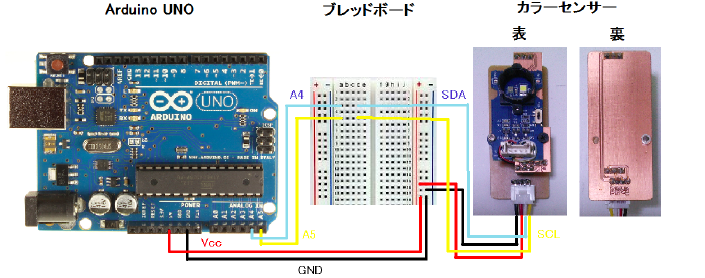
\includegraphics[width=7.0cm]{images/enshu8-1-1.png}
\caption{演習8.1.1の回路}
\label{fig:enshu8-1-1}
\end{center}
\end{figure}

\subsection{演習8.1.2}
Arduinoで,$I^2-C$による通信を実行するためのWire関数の使い方について理解した.

以下ソースコード\ref{code:enshu8-1-2-a}に作成したプログラムのソースコードを示す.

\lstinputlisting[caption = 演習8.1.2(Arduino),label=code:enshu8-1-2-a]{enshu8-1-2.ino}

\subsection{演習8.1.3}
演習8.1.2で取得したカラーセンサの値をProcessingで可視化した.

以下ソースコード\ref{code:enshu8-1-3-p}に作成したプログラムのソースコードを示す.

\lstinputlisting[caption = 演習8.1.3(Processing),label=code:enshu8-1-3-p]{enshu8_1_3.pde}

\subsection{演習8.1.4}
フルカラーLEDにより基本色であるRGBを再現した.
以下図\ref{fig:enshu8-1-4}にブレッドボード上の構成図を示す.

\begin{figure}[H]
\begin{center}
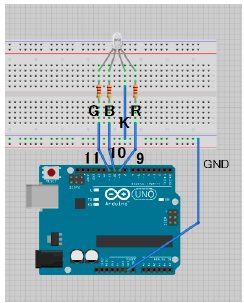
\includegraphics[width=7.0cm]{images/enshu8-1-4.png}
\caption{演習8.1.4の配線図}
\label{fig:enshu8-1-4}
\end{center}
\end{figure}

\subsection{演習8.1.5}
カラーセンサによりフルカラーLEDの値を読み出しシリアルモニタに表示するプログラムを作成した.ただし同期タイミングを合わせるため,タイマ割り込みを用いた.
以下ソースコード\ref{code:enshu8-1-5-a}に作成したプログラムのソースコードを示す.

\lstinputlisting[caption = 演習8.1.5(Arduino),label=code:enshu8-1-5-a]{enshu8-1-5-2.ino}

\subsection{演習8.1.6}
RGB値からxy値に変換するためのプログラムを作成した.
ここで変換行列に
\begin{equation}
A = 
\begin{pmatrix}
-0.142 & 1.549 & -0.956 \\
-0.334 & 1.578 & -0.731 \\
-0.682 & 0.770 & 0.563 
\end{pmatrix}
\end{equation}

を用いた.
以下ソースコード\ref{code:enshu8-1-6-a}に作成したプログラムのソースコードを示す.

\lstinputlisting[caption = 演習8.1.6(Arduino),label=code:enshu8-1-6-a]{enshu8-1-6.ino}

\section{課題}
\subsection{課題8.1.1}
演習8.1.3で作成したプログラムを元に,Clear値についても可視化した.\\
また,カラーセンサの値を読み取る通信速度についても検討した.これについてはタイマー割り込みを用いて同期させることで改善した.

以下ソースコード\ref{code:kadai8-1-1-a},\ref{code:kadai8-1-1-p}にそれぞれ作成したプログラムのソースコードを示す.

\lstinputlisting[caption = 課題8.1.1(Arduino),label=code:kadai8-1-1-a]{kadai8-1-1.ino}

\lstinputlisting[caption = 課題8.1.1(Processing),label=code:kadai8-1-1-p]{kadai8_1_1.pde}


\subsection{課題8.1.2}
演習8.1.5のスケッチを元に,Green,Blueを加えまた,シアン,マゼンタ,イエローを表現するプログラムを完成させた.

以下ソースコード\ref{code:kadai8-1-2-a}に作成したプログラムのソースコードを示す.

\lstinputlisting[caption = 課題8.1.2(Arduino),label=code:kadai8-1-2-a]{kadai8-1-2.ino}

結果としては,青と赤でマゼンタ,青と緑でシアン,赤と緑でイエローがそれぞれフルカラーLEDの出力として得られた.

\subsection{課題8.1.3}
取得したカラーセンサのRGB値をXYZ値に変換後,xy色度図上に投影した.ただしオートキャリブレーションを行い,あらかじめキャリブレーションはするものとした.


以下ソースコード\ref{code:kadai8-1-3-a},\ref{code:kadai8-1-3-p}にそれぞれ作成したプログラムのソースコードを示す.

\lstinputlisting[caption = 課題8.1.3(Arduino),label=code:kadai8-1-3-a]{kadai8-1-3_kaizen.ino}

\lstinputlisting[caption = 課題8.1.3(Processing),label=code:kadai8-1-3-p]{kadai8_1_3.pde}

また,以下図\ref{fig:kadai8-1-3}にプログラムの実行結果の図を示す.

\begin{figure}[H]
\begin{center}
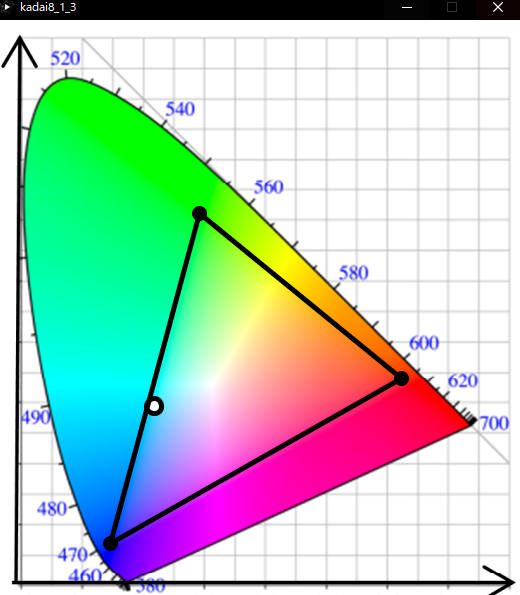
\includegraphics[width=7.0cm]{images/kadai8-1-3.png}
\caption{課題8.1.3の実行結果}
\label{fig:kadai8-1-3}
\end{center}
\end{figure}

\subsection{課題8.1.4}
取得したカラーセンサのRGB値をXYZ値に変換後,xy色度図上に投影した.ただしオートキャリブレーションを行わず,あらかじめカラーセンサの値を用いてマニュアルキャリブレーションするものとした.


以下ソースコード\ref{code:kadai8-1-4-a},\ref{code:kadai8-1-4-p}にそれぞれ作成したプログラムのソースコードを示す.

\lstinputlisting[caption = 課題8.1.4(Arduino),label=code:kadai8-1-4-a]{kadai8-1-4.ino}

\lstinputlisting[caption = 課題8.1.4(Processing),label=code:kadai8-1-4-p]{kadai8_1_3.pde}

また,以下図\ref{fig:kadai8-1-4}にプログラムの実行結果の図を示す.

\begin{figure}[H]
\begin{center}
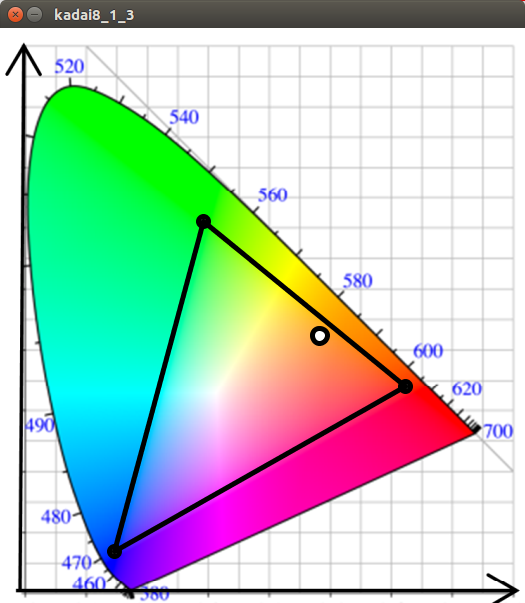
\includegraphics[width=7.0cm]{images/kadai8-1-4.png}
\caption{課題8.1.4の実行結果}
\label{fig:kadai8-1-4}
\end{center}
\end{figure}

正直課題8.1.3と課題8.1.4であまり違いがでなかった.キャリブレーションがうまくいっていないのか青や赤をセンシングしてもそれに近いところまでいかず中間の値で止まっていた.

\subsection{課題8.1.5}
色をセンシングしてから表示するまでにかかる内部処理の時間をmillis関数を用いて計測した.
以下ソースコード\ref{code:kadai8-1-5-a}に作成したプログラムのソースコードを示す.

\lstinputlisting[caption = 課題8.1.5(Arduino),label=code:kadai8-1-5-a]{./Processing/kadai8-1-5/kadai8-1-5.ino}

計測すると大体200$\sim$203msだった.これより,計測に200msかかると考えると,センシングのタイミング(サンプリング周期)は400ms以上にするべきだと考えられる.

\end{document}
